\begin{frame}[t]
\begin{columns}[t]
\separatorcolumn

\begin{column}{\colwidth}

  \begin{block}{A block title}

    Some block contents, followed by a diagram, followed by a dummy paragraph.

    \begin{figure}
      \centering
      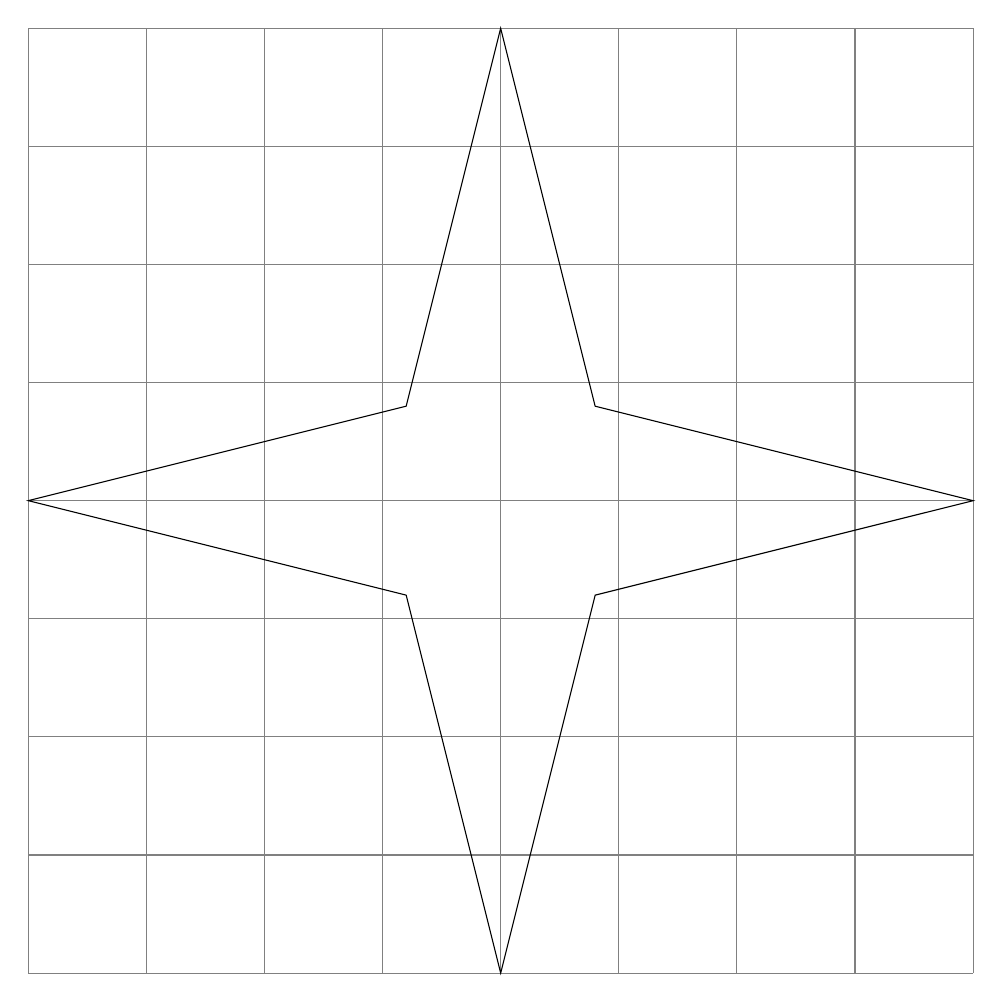
\begin{tikzpicture}[scale=6]
        \draw[step=0.25cm,color=gray] (-1,-1) grid (1,1);
        \draw (1,0) -- (0.2,0.2) -- (0,1) -- (-0.2,0.2) -- (-1,0)
          -- (-0.2,-0.2) -- (0,-1) -- (0.2,-0.2) -- cycle;
      \end{tikzpicture}
      \caption{A figure caption.}
    \end{figure}

    Lorem ipsum dolor sit amet, consectetur adipiscing elit. Morbi ultricies
    eget libero ac ullamcorper. Integer et euismod ante. Aenean vestibulum
    lobortis augue, ut lobortis turpis rhoncus sed. Proin feugiat nibh a
    lacinia dignissim. Proin scelerisque, risus eget tempor fermentum, ex
    turpis condimentum urna, quis malesuada sapien arcu eu purus.

  \end{block}


\end{column}

\separatorcolumn

\begin{column}{\colwidth}





\end{column}

\separatorcolumn

\begin{column}{\colwidth}

  \begin{block}{A block containing some math}

    Nullam non est elit. In eu ornare justo. Maecenas porttitor sodales lacus,
    ut cursus augue sodales ac.

    $$
    \int_{-\infty}^{\infty} e^{-x^2}\,dx = \sqrt{\pi}
    $$

    Interdum et malesuada fames $\{1, 4, 9, \ldots\}$ ac ante ipsum primis in
    faucibus. Cras eleifend dolor eu nulla suscipit suscipit. Sed lobortis non
    felis id vulputate.

    \heading{A heading inside a block}

    Praesent consectetur mi $x^2 + y^2$ metus, nec vestibulum justo viverra
    nec. Proin eget nulla pretium, egestas magna aliquam, mollis neque. Vivamus
    dictum $\mathbf{u}^\intercal\mathbf{v}$ sagittis odio, vel porta erat
    congue sed. Maecenas ut dolor quis arcu auctor porttitor.

    \heading{Another heading inside a block}

    Sed augue erat, scelerisque a purus ultricies, placerat porttitor neque.
    Donec $P(y \mid x)$ fermentum consectetur $\nabla_x P(y \mid x)$ sapien
    sagittis egestas. Duis eget leo euismod nunc viverra imperdiet nec id
    justo.

  \end{block}


  \begin{block}{References}

    \nocite{*}
    \footnotesize{\bibliographystyle{plain}\bibliography{poster}}

  \end{block}

\end{column}

\separatorcolumn
\end{columns}
\end{frame}
